\header{
    \section{Le pou et l'araignée} \label{le-pou-et-l-araignee}
    %
    \insertComment{Publiée en 1911 dans l'Anthologie hospitalière et latinesque. Paroles de Musset et musique probablement de Berlioz.}{Brassens y fait référence des les Quat'z'arts.}
}

\enluminure{2}{\href{https://www.youtube.com/watch?v=YlDQiQGg08Q}{U}}{n pou} s' baladait dans la rue,
\\Il rencontra chemin faisant,
\\Chemin faisant,
\\Une araignée bon enfant
\\Qui s'en allait court vêtue;
\\Ell' vendait du verr' pilé,
\\Pour s'ach'ter des p'tits souliers.
\\\\\textbf{Refrain :}
\\Là tu, là tu m'emmerdes
\\Là tu,là tu m' fais chier
\\Tu nous emmerdes
\\Tu nous fais chier
\\Tu nous emmerdes
\\Tu nous fais chier
\\Et on entend dans les champs
\\Se masturber les éléphants,
\\Et on entend dans les prés,
\\Gazouiller les chimpanzés,
\\Et on entend sous les ormeaux
\\Battr' la merde à coup d' marteaux,
\\Et on entend dans les plumards
\\Battr' le foutre à coup d' braquemarts.
\\Non, non,non, non, Saint Eloi n'est pas mort \bissimple
\\Car il bande encore \bissimple
\\\\Le pou voulait la séduire
\\L'emm'na chez l' mastroquet du coin,
\\Troquet du coin,
\\Lui fit boir' cinq, six coup's de vin,
\\L'araignée ne fit qu'en rire.
\\La pauvrett' ne s' doutait pas
\\Qu'ell' courait à son trépas.
\\\\Le pou lui offrit une prise
\\En lui disant d'un air joyeux,
\\D'un air joyeux,
\\Fous-toi ça dans les narines
\\Et mouch'-toi avec ta ch'mise.
\\L'araignée qu'en avait pas
\\Lui fit voir tous ses appas.
\\\\Le pou qui n'était qu'un' canaille
\\Lui offrit trois francs six sous,
\\Trois francs six sous:
\\"Eh! Dis donc, c'est pas l' Pérou
\\Ca ne me dit rien qui vaille,
\\Si tu m' donn's quatr' sous de plus
\\J' te ferai voir le trou d' mon cul".
\\\\C'est ici qu' les horreurs commencent
\\Le pou grimpa sur l'araignée,
\\Sur l'araignée
\\Et n' put s'en décoller
\\Tant il eut de jouissance,
\\Si bien qu' la pauvre araignée
\\Ecop' d' la maternité.
\\\\Le pèr' d' l'araignée en colère
\\Lui dit: "Tu m'as déshonoré,
\\Déshonoré,
\\Tu t'es laissée enceinter,
\\T'es aussi putain qu' ta mère!"
\\L'araignée de désespoir
\\S'est foutu treiz' coups d' rasoir.
\\\\Le pou, le désespoir dans l'âme,
\\S'arracha des poignées d' cheveux,
\\Poignées d' cheveux
\\Puis disant: "Y a plus d' Bon Dieu",
\\Il monta à Notre-Dame
\\Et c'est là qu'il s'est foutu
\\Les cinq doigts et l' pouc' dans l' cul.
\breakpage
\\\\Alors, les poux du voisinage
\\Se réunir'nt pour l'enterrer,
\\Pour l'enterrer
\\Au cim'tièr' de Champerret
\\Tout comme un grand personnage
\\Et c'était bien triste à voir
\\Tous ces poux en habit noir!
\\\\
\bigskip
\begin{center}
   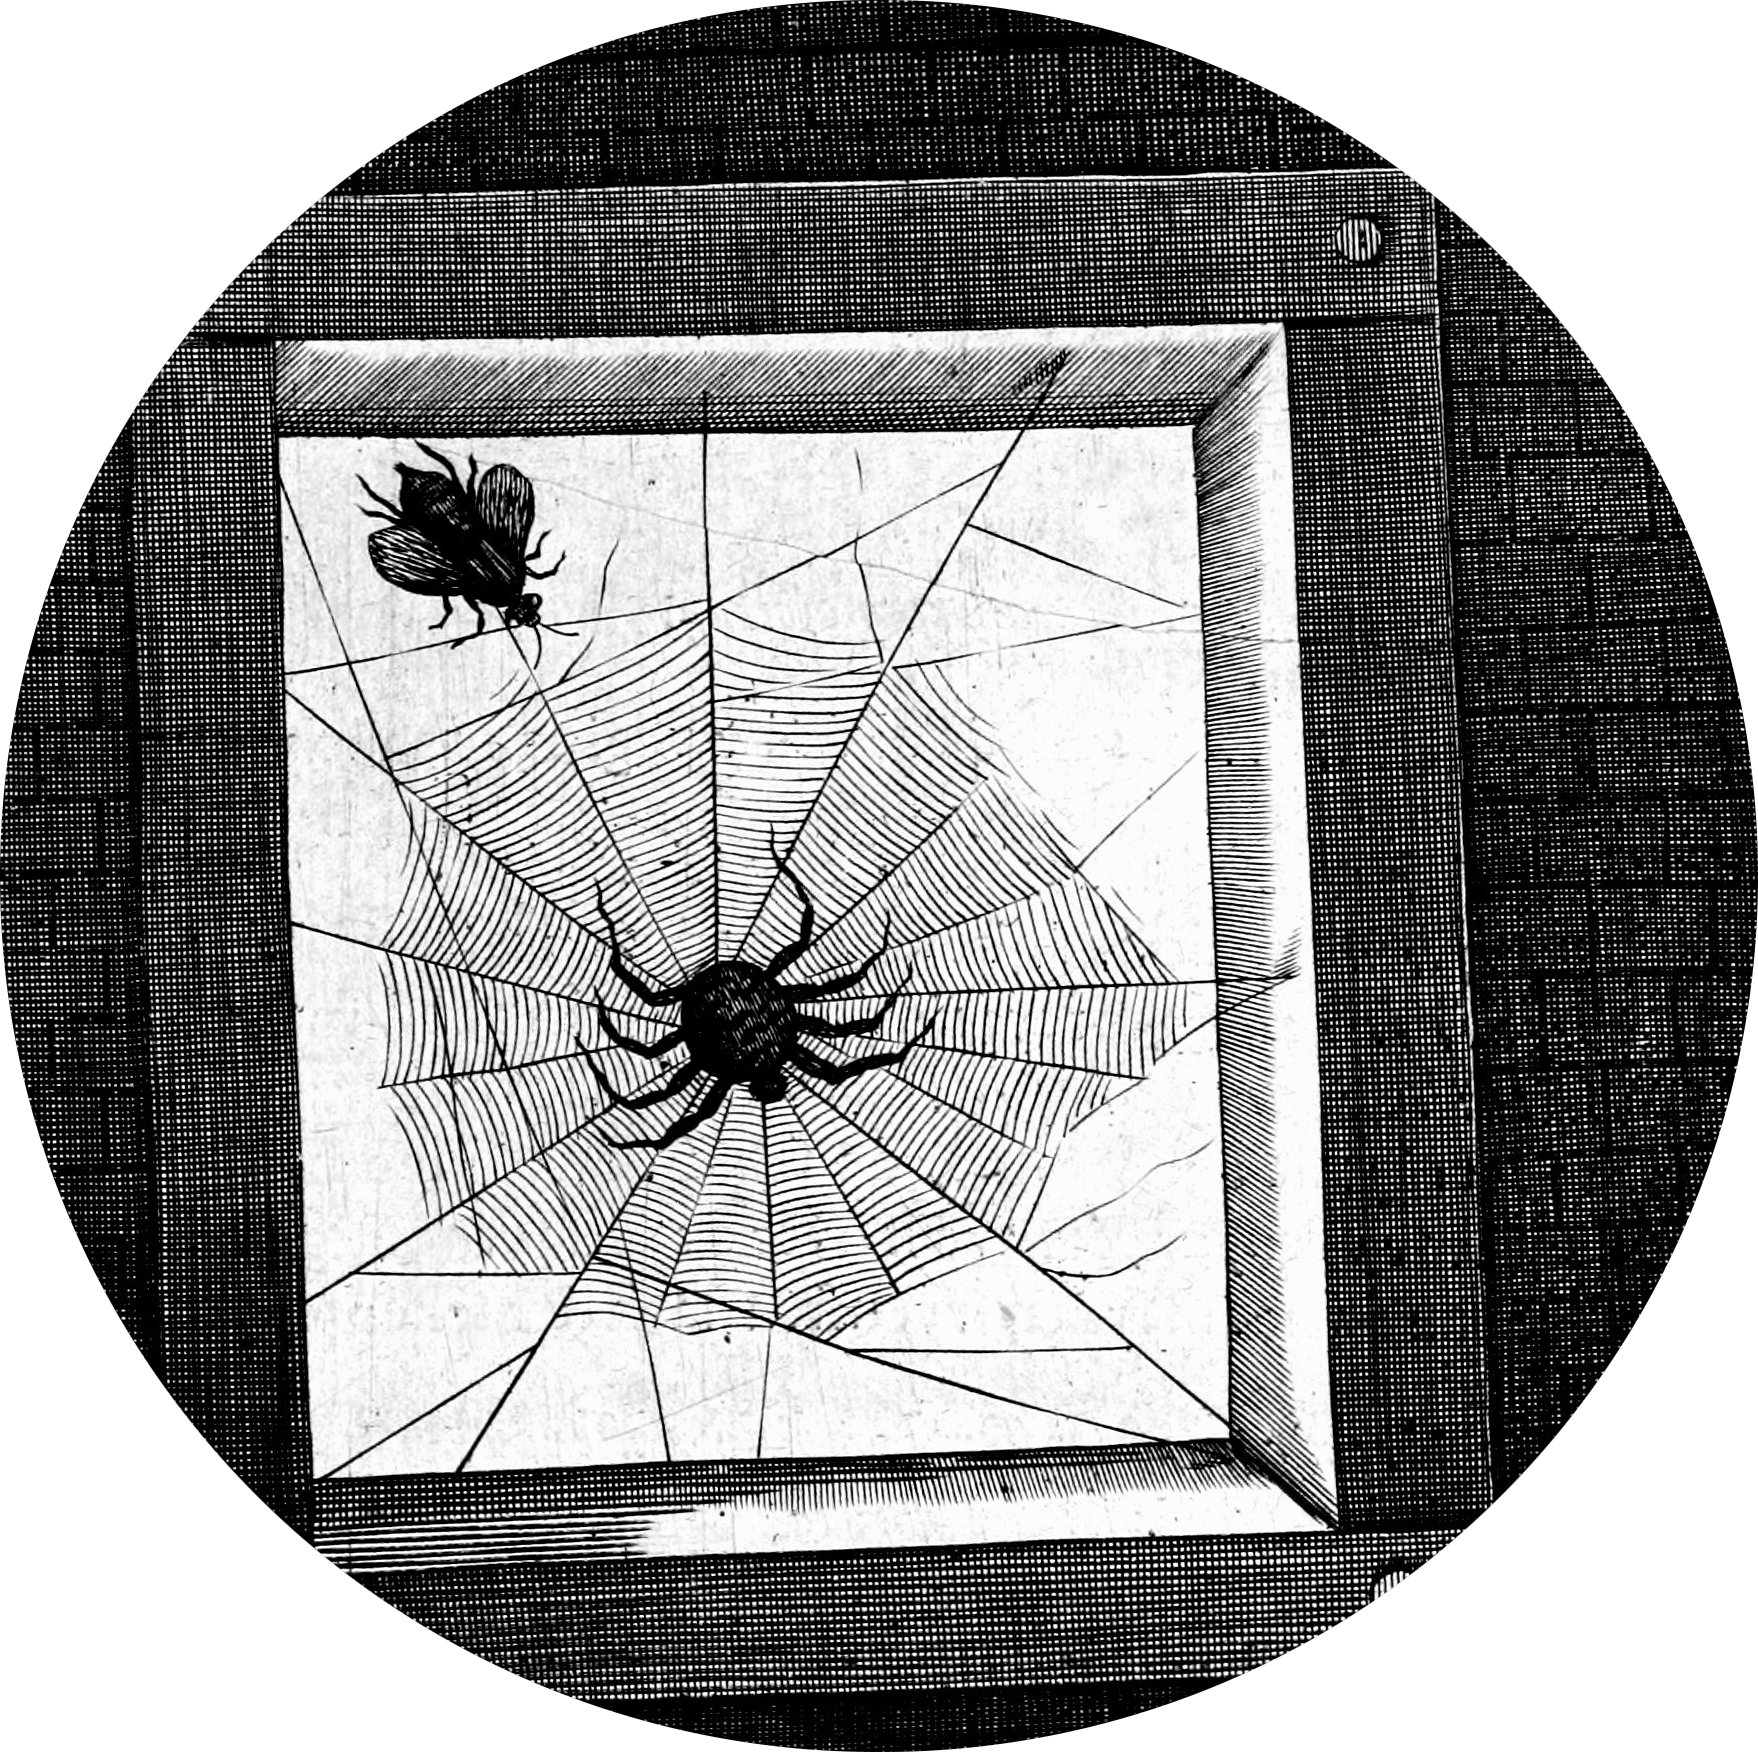
\includegraphics[width=1\textwidth]{images/brev32.png}
 \end{center}


\breakpage